% Options for packages loaded elsewhere
\PassOptionsToPackage{unicode}{hyperref}
\PassOptionsToPackage{hyphens}{url}
\PassOptionsToPackage{dvipsnames,svgnames*,x11names*}{xcolor}
%
\documentclass[
  english,
  man,floatsintext]{apa6}
\usepackage{lmodern}
\usepackage{amssymb,amsmath}
\usepackage{ifxetex,ifluatex}
\ifnum 0\ifxetex 1\fi\ifluatex 1\fi=0 % if pdftex
  \usepackage[T1]{fontenc}
  \usepackage[utf8]{inputenc}
  \usepackage{textcomp} % provide euro and other symbols
\else % if luatex or xetex
  \usepackage{unicode-math}
  \defaultfontfeatures{Scale=MatchLowercase}
  \defaultfontfeatures[\rmfamily]{Ligatures=TeX,Scale=1}
\fi
% Use upquote if available, for straight quotes in verbatim environments
\IfFileExists{upquote.sty}{\usepackage{upquote}}{}
\IfFileExists{microtype.sty}{% use microtype if available
  \usepackage[]{microtype}
  \UseMicrotypeSet[protrusion]{basicmath} % disable protrusion for tt fonts
}{}
\makeatletter
\@ifundefined{KOMAClassName}{% if non-KOMA class
  \IfFileExists{parskip.sty}{%
    \usepackage{parskip}
  }{% else
    \setlength{\parindent}{0pt}
    \setlength{\parskip}{6pt plus 2pt minus 1pt}}
}{% if KOMA class
  \KOMAoptions{parskip=half}}
\makeatother
\usepackage{xcolor}
\IfFileExists{xurl.sty}{\usepackage{xurl}}{} % add URL line breaks if available
\IfFileExists{bookmark.sty}{\usepackage{bookmark}}{\usepackage{hyperref}}
\hypersetup{
  pdftitle={Epidemiologische situatie COVID-19 in Nederland - 21 oktober 2020},
  pdfauthor={Marino van Zelst1},
  pdflang={en-EN},
  colorlinks=true,
  linkcolor=Maroon,
  filecolor=Maroon,
  citecolor=Blue,
  urlcolor=blue,
  pdfcreator={LaTeX via pandoc}}
\urlstyle{same} % disable monospaced font for URLs
\usepackage{graphicx,grffile}
\makeatletter
\def\maxwidth{\ifdim\Gin@nat@width>\linewidth\linewidth\else\Gin@nat@width\fi}
\def\maxheight{\ifdim\Gin@nat@height>\textheight\textheight\else\Gin@nat@height\fi}
\makeatother
% Scale images if necessary, so that they will not overflow the page
% margins by default, and it is still possible to overwrite the defaults
% using explicit options in \includegraphics[width, height, ...]{}
\setkeys{Gin}{width=\maxwidth,height=\maxheight,keepaspectratio}
% Set default figure placement to htbp
\makeatletter
\def\fps@figure{htbp}
\makeatother
\setlength{\emergencystretch}{3em} % prevent overfull lines
\providecommand{\tightlist}{%
  \setlength{\itemsep}{0pt}\setlength{\parskip}{0pt}}
\setcounter{secnumdepth}{-\maxdimen} % remove section numbering
% Make \paragraph and \subparagraph free-standing
\ifx\paragraph\undefined\else
  \let\oldparagraph\paragraph
  \renewcommand{\paragraph}[1]{\oldparagraph{#1}\mbox{}}
\fi
\ifx\subparagraph\undefined\else
  \let\oldsubparagraph\subparagraph
  \renewcommand{\subparagraph}[1]{\oldsubparagraph{#1}\mbox{}}
\fi
% Manuscript styling
\usepackage{upgreek}
\captionsetup{font=singlespacing,justification=justified}

% Table formatting
\usepackage{longtable}
\usepackage{lscape}
% \usepackage[counterclockwise]{rotating}   % Landscape page setup for large tables
\usepackage{multirow}		% Table styling
\usepackage{tabularx}		% Control Column width
\usepackage[flushleft]{threeparttable}	% Allows for three part tables with a specified notes section
\usepackage{threeparttablex}            % Lets threeparttable work with longtable

% Create new environments so endfloat can handle them
% \newenvironment{ltable}
%   {\begin{landscape}\begin{center}\begin{threeparttable}}
%   {\end{threeparttable}\end{center}\end{landscape}}
\newenvironment{lltable}{\begin{landscape}\begin{center}\begin{ThreePartTable}}{\end{ThreePartTable}\end{center}\end{landscape}}

% Enables adjusting longtable caption width to table width
% Solution found at http://golatex.de/longtable-mit-caption-so-breit-wie-die-tabelle-t15767.html
\makeatletter
\newcommand\LastLTentrywidth{1em}
\newlength\longtablewidth
\setlength{\longtablewidth}{1in}
\newcommand{\getlongtablewidth}{\begingroup \ifcsname LT@\roman{LT@tables}\endcsname \global\longtablewidth=0pt \renewcommand{\LT@entry}[2]{\global\advance\longtablewidth by ##2\relax\gdef\LastLTentrywidth{##2}}\@nameuse{LT@\roman{LT@tables}} \fi \endgroup}

% \setlength{\parindent}{0.5in}
% \setlength{\parskip}{0pt plus 0pt minus 0pt}

% \usepackage{etoolbox}
\makeatletter
\patchcmd{\HyOrg@maketitle}
  {\section{\normalfont\normalsize\abstractname}}
  {\section*{\normalfont\normalsize\abstractname}}
  {}{\typeout{Failed to patch abstract.}}
\patchcmd{\HyOrg@maketitle}
  {\section{\protect\normalfont{\@title}}}
  {\section*{\protect\normalfont{\@title}}}
  {}{\typeout{Failed to patch title.}}
\makeatother
\shorttitle{Dagelijkse rapportage}
\DeclareDelayedFloatFlavor{ThreePartTable}{table}
\DeclareDelayedFloatFlavor{lltable}{table}
\DeclareDelayedFloatFlavor*{longtable}{table}
\makeatletter
\renewcommand{\efloat@iwrite}[1]{\immediate\expandafter\protected@write\csname efloat@post#1\endcsname{}}
\makeatother
\usepackage{csquotes}
\ifxetex
  % Load polyglossia as late as possible: uses bidi with RTL langages (e.g. Hebrew, Arabic)
  \usepackage{polyglossia}
  \setmainlanguage[]{english}
\else
  \usepackage[shorthands=off,main=english]{babel}
\fi

\title{Epidemiologische situatie COVID-19 in Nederland - 21 oktober 2020}
\author{Marino van Zelst\textsuperscript{1}}
\date{}


\affiliation{\vspace{0.5cm}\textsuperscript{1} Vragen over deze rapportage kunnen verstuurd worden aan Marino van Zelst, twitter.com/mzelst. E-mail: \href{mailto:j.m.vanzelst@uvt.nl}{\nolinkurl{j.m.vanzelst@uvt.nl}}}

\begin{document}
\maketitle

{
\hypersetup{linkcolor=}
\setcounter{tocdepth}{3}
\tableofcontents
}
\newpage

\hypertarget{samenvatting}{%
\section{Samenvatting}\label{samenvatting}}

\textbf{Samenvatting}\\
<<<<<<< HEAD
Tot en met 2020-09-06 zijn er in Nederland in totaal 74787 COVID-19 patiënten gemeld aan het RIVM. Van alle gemelde patiënten is de helft 55 jaar of ouder. Tot nu toe zijn 12210 van de gemelde patiënten opgenomen in het ziekenhuis en 6243 mensen overleden.

\textbf{Gegevens t. o. v. gisteren}\\
Positief getest: 945
Totaal: 74787 (+ 925 ivm -20 corr.)

Opgenomen: 5
Totaal: 12210 (+
5 ivm 0 corr.)
=======
Tot en met 2020-10-21 zijn er in Nederland in totaal 253134 COVID-19 patiënten gemeld aan het RIVM. Van alle gemelde patiënten is de helft 55 jaar of ouder. Tot nu toe zijn 14130 van de gemelde patiënten opgenomen in het ziekenhuis en 6873 mensen overleden.

\textbf{Gegevens t. o. v. gisteren}\\
Positief getest: 8788
Totaal: 253134 (+ 8743 ivm -45 corr.)

Opgenomen: 101
Totaal: 14130 (+
101 ivm 0 corr.)
>>>>>>> 5b9eaab0334e6c06a82cf82b892a3e99c7341e30

Opgenomen op IC: 6
Totaal: 3994

<<<<<<< HEAD
Overleden: 2
Totaal: 6243 (+
2 ivm 0 corr.)
=======
Overleden: 60
Totaal: 6873 (+
59 ivm -1 corr.)
>>>>>>> 5b9eaab0334e6c06a82cf82b892a3e99c7341e30

\textbf{Update met betrekking tot ziekenhuis-gegevens (data NICE)}

Patiënten verpleegafdeling\\
Bevestigd: 20 Verdacht: 15

Patiënten IC\\
Bevestigd: 17 Verdacht: 2

\textbf{Data}\\
Een databestand met de cumulatieve aantallen per gemeente per dag van gemelde COVID-19 patiënten, in het ziekenhuis opgenomen COVID-19 patiënten en overleden COVID-19 patiënten is \href{https://data.rivm.nl/geonetwork/srv/dut/catalog.search\#/metadata/1c0fcd57-1102-4620-9cfa-441e93ea5604}{hier} te vinden. Een databestand met karakteristieken van elke positief geteste COVID-19 patiënt in Nederland is \href{https://data.rivm.nl/geonetwork/srv/dut/catalog.search\#/metadata/2c4357c8-76e4-4662-9574-1deb8a73f724?tab=relations}{hier} te vinden. Alle gegevens die voor dit rapport gebruikt worden zijn te vinden in de \href{https://github.com/mzelst/covid-19}{Github repository}.

\newpage

\hypertarget{covid-19-meldingen-in-de-afgelopen-vier-weken}{%
\section{COVID-19 meldingen in de afgelopen vier weken}\label{covid-19-meldingen-in-de-afgelopen-vier-weken}}

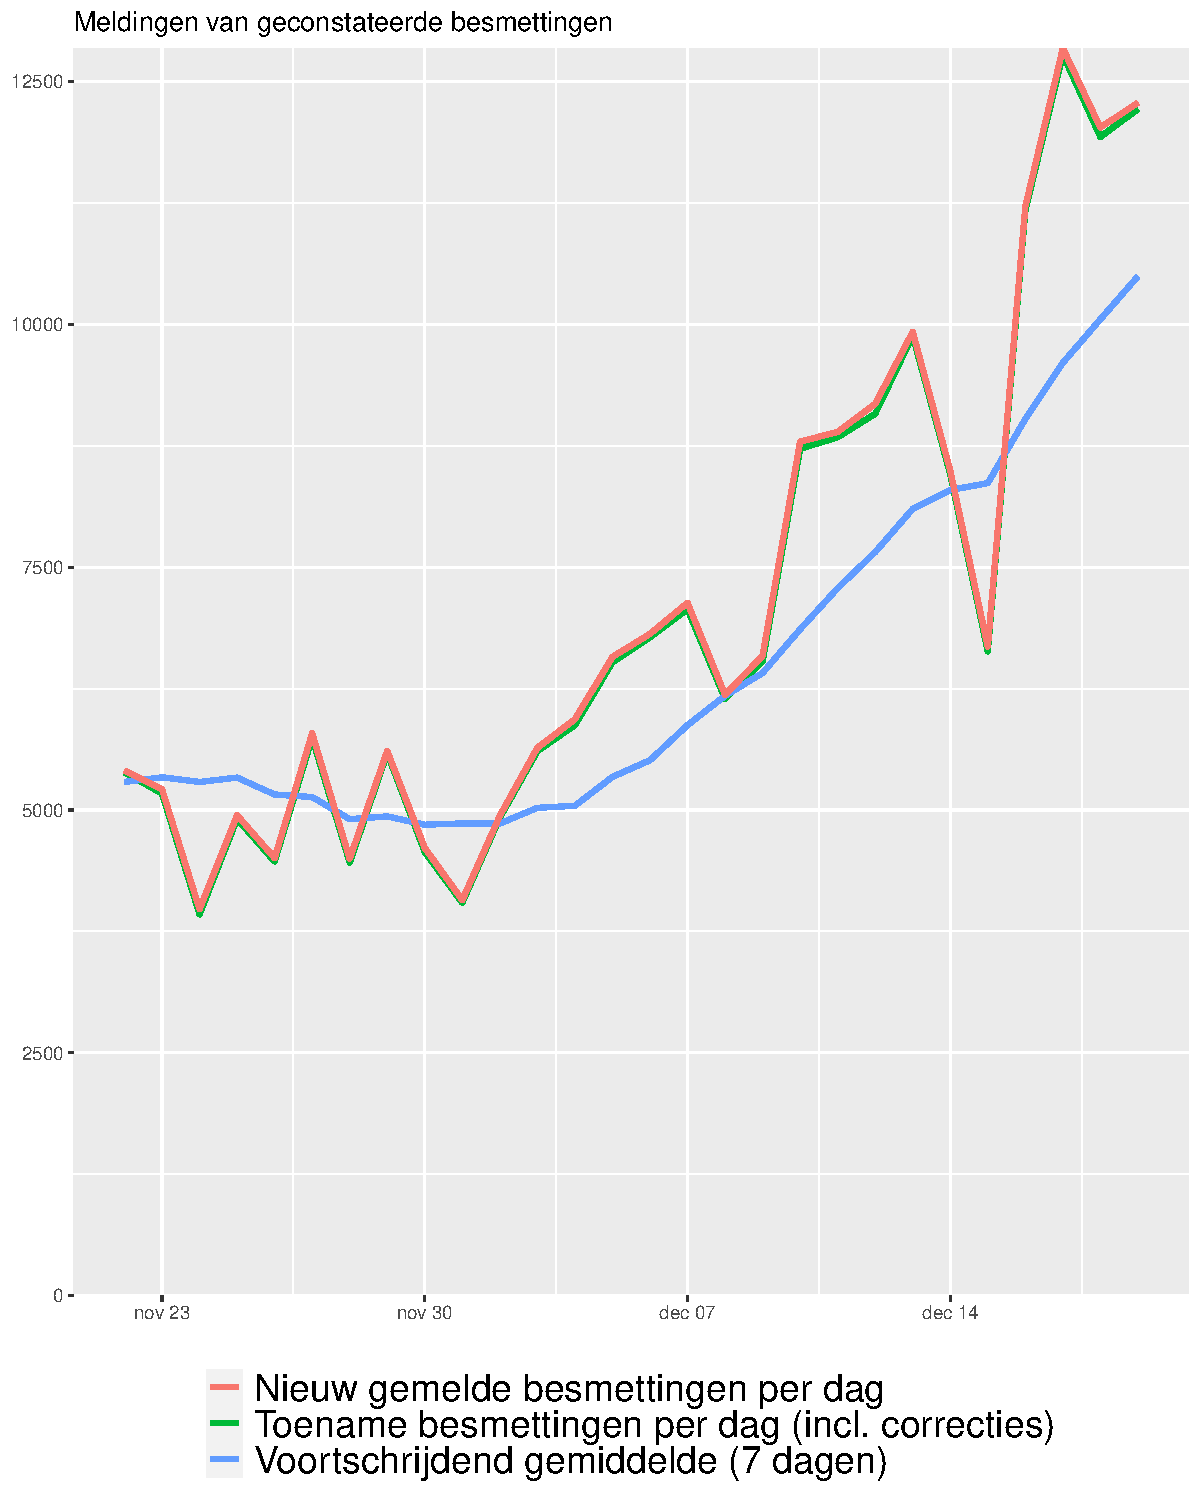
\includegraphics{daily_report_files/figure-latex/Gemelde besmettingen-1.pdf}

\newpage

\hypertarget{kaart-met-covid-19-meldingen-per-gemeente-sinds-gisteren}{%
\section{Kaart met COVID-19 meldingen per gemeente sinds gisteren}\label{kaart-met-covid-19-meldingen-per-gemeente-sinds-gisteren}}

\begin{figure}
\centering
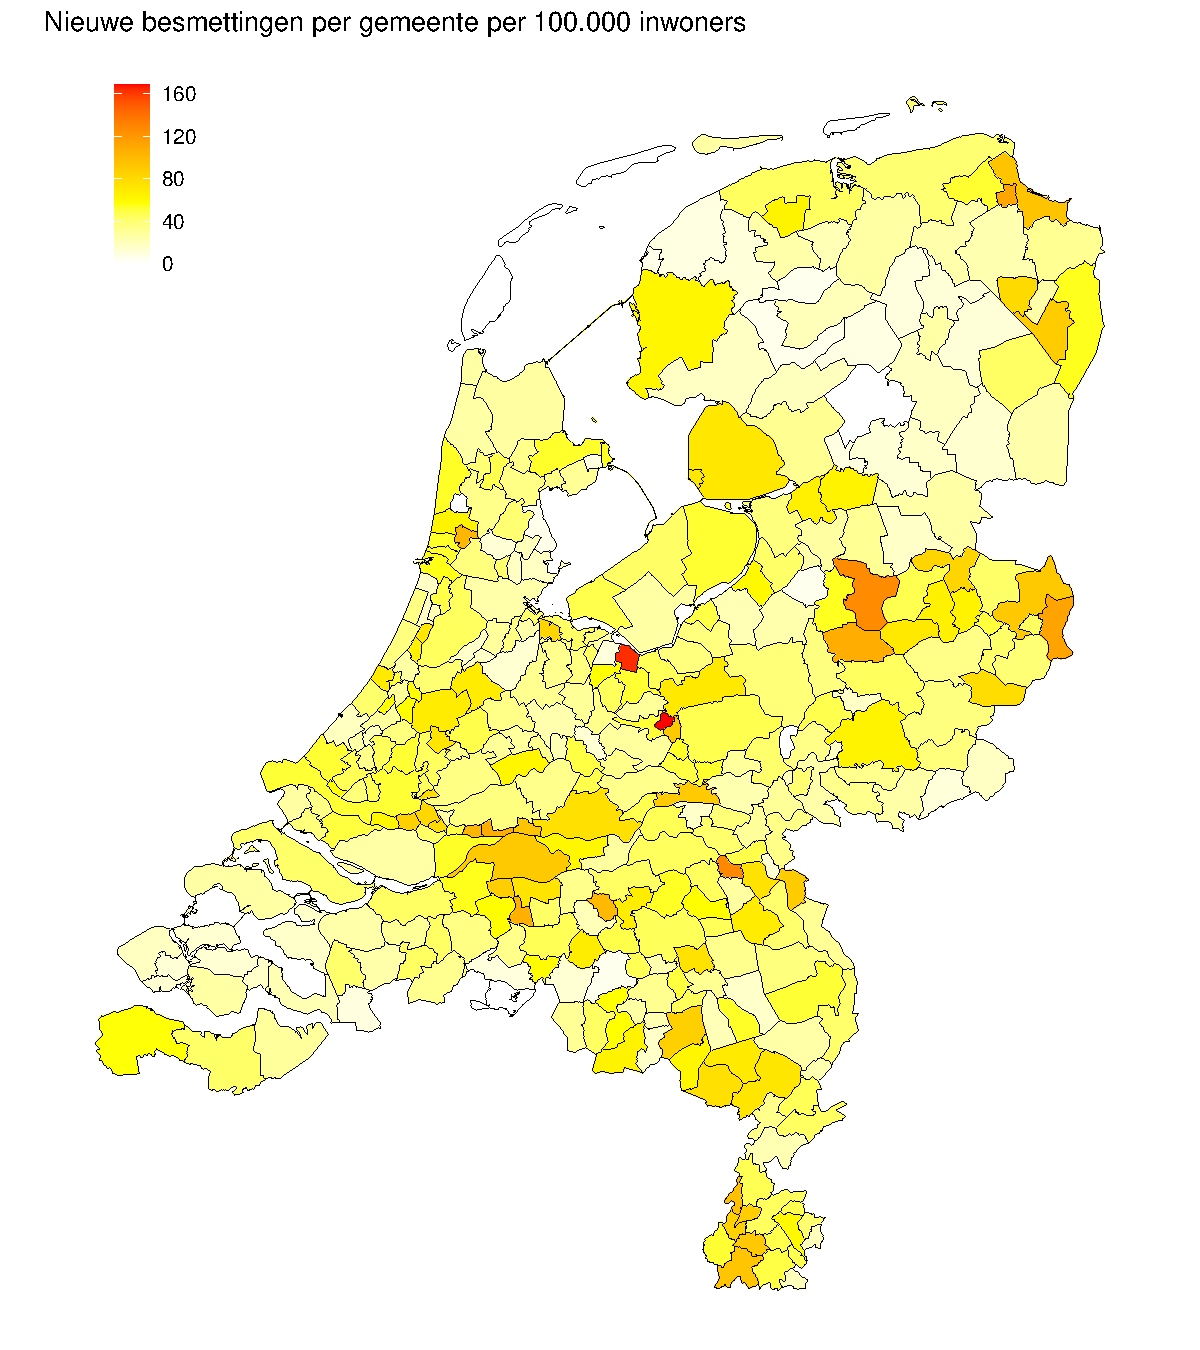
\includegraphics{daily_report_files/figure-latex/Gemeentes - sinds gisteren-1.pdf}
\caption{(\#Gemeentes - sinds gisteren) Aantal, sinds gisteren, bij de GGD'en gemelde COVID-19 patiënten per 100.000 inwoners per gemeente}
\end{figure}

\newpage

\hypertarget{kaart-met-covid-19-meldingen-per-gemeente-in-de-afgelopen-week}{%
\section{Kaart met COVID-19 meldingen per gemeente in de afgelopen week}\label{kaart-met-covid-19-meldingen-per-gemeente-in-de-afgelopen-week}}

\begin{figure}
\centering
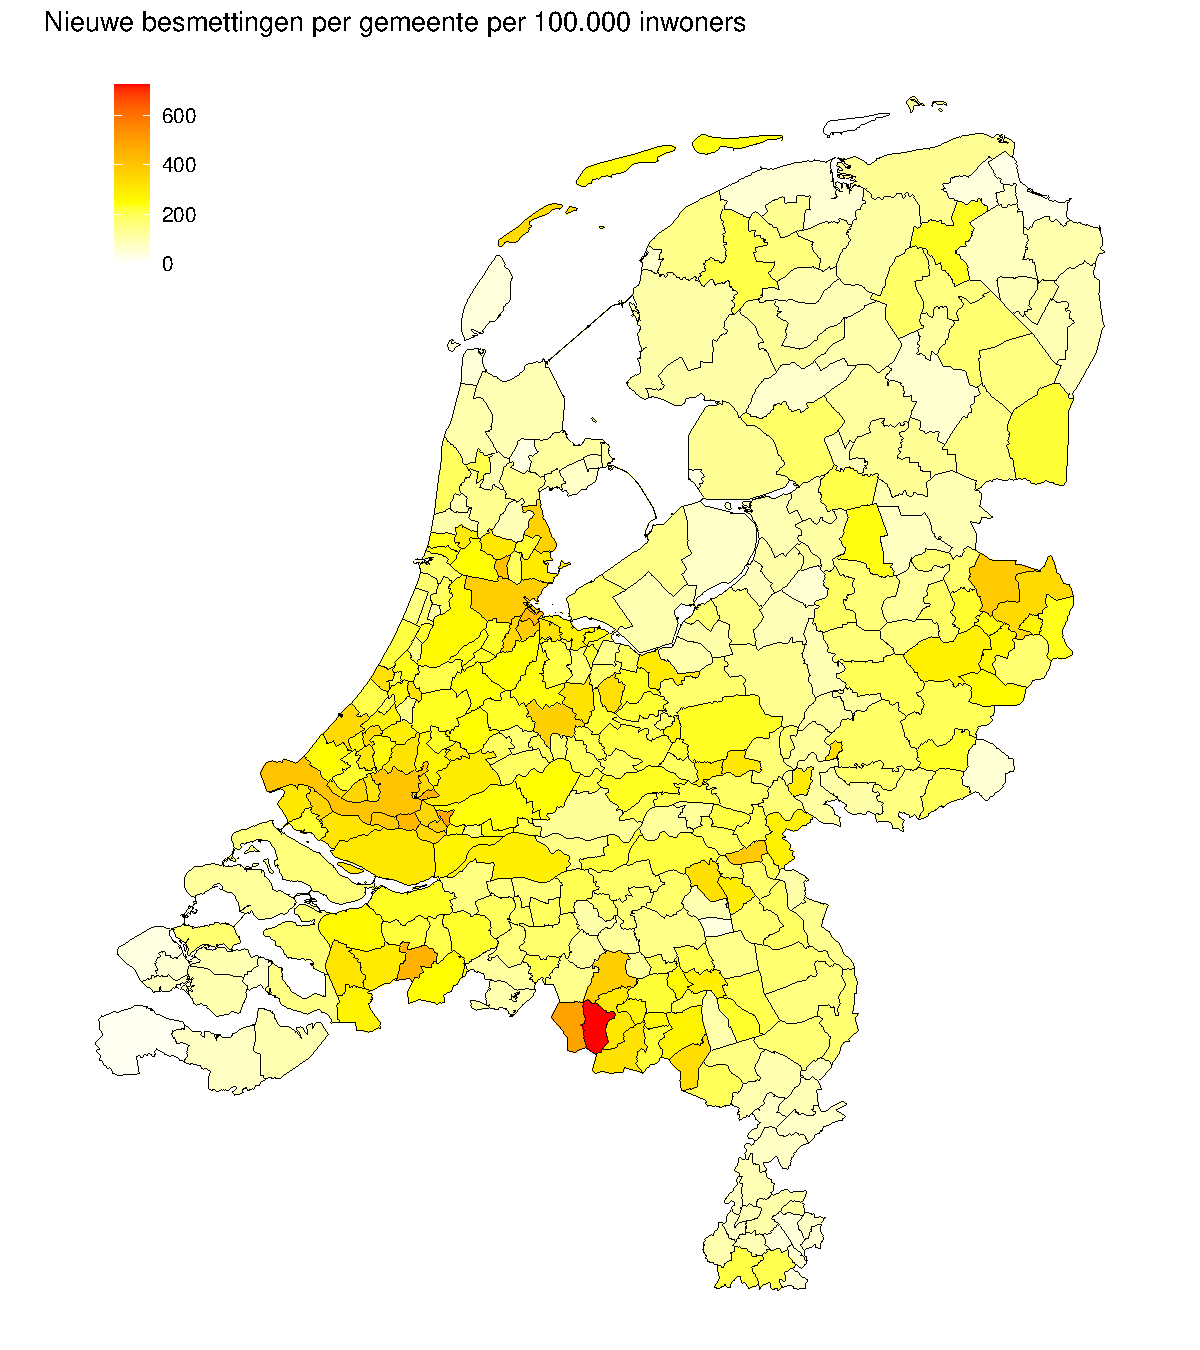
\includegraphics{daily_report_files/figure-latex/Gemeentes - Sinds vorige week-1.pdf}
\caption{(\#Gemeentes - Sinds vorige week) Aantal in de afgelopen week bij de GGD'en gemelde COVID-19 patiënten per 100.000 inwoners per gemeente.}
\end{figure}

\newpage

\hypertarget{aantal-covid-19-meldingen-per-provincie-in-de-afgelopen-twee-weken}{%
\section{Aantal COVID-19 meldingen per provincie in de afgelopen twee weken}\label{aantal-covid-19-meldingen-per-provincie-in-de-afgelopen-twee-weken}}

\begin{table}[H]
\centering
\begin{threeparttable}
\begin{tabular}{lrrrrrr}
\toprule
\multicolumn{1}{c}{ } & \multicolumn{2}{c}{Besmettingen} & \multicolumn{2}{c}{Ziekenhuisopnames} & \multicolumn{2}{c}{Overleden} \\
\cmidrule(l{3pt}r{3pt}){2-3} \cmidrule(l{3pt}r{3pt}){4-5} \cmidrule(l{3pt}r{3pt}){6-7}
Provincie & Totaal & /100000 & Totaal & /100000 & Totaal & /100000\\
\midrule
<<<<<<< HEAD
Drenthe & 21 & 4.3 & 0 & 0.0 & 0 & 0.0\\
Flevoland & 167 & 39.5 & 1 & 0.2 & 2 & 0.5\\
Friesland & 62 & 9.5 & 1 & 0.2 & 0 & 0.0\\
Gelderland & 556 & 26.7 & 2 & 0.1 & 3 & 0.1\\
Groningen & 77 & 13.1 & 1 & 0.2 & 2 & 0.3\\
Limburg & 311 & 27.8 & 5 & 0.4 & 2 & 0.2\\
Noord-Brabant & 1063 & 41.5 & 8 & 0.3 & 4 & 0.2\\
Noord-Holland & 2184 & 75.8 & 29 & 1.0 & 7 & 0.2\\
Overijssel & 168 & 14.5 & 3 & 0.3 & 2 & 0.2\\
Utrecht & 668 & 49.3 & 8 & 0.6 & 5 & 0.4\\
Zeeland & 70 & 18.3 & 0 & 0.0 & 3 & 0.8\\
Zuid-Holland & 2886 & 77.8 & 45 & 1.2 & 13 & 0.4\\
=======
Drenthe & 2205 & 446.6 & 35 & 7.1 & 11 & 2.2\\
Flevoland & 1788 & 422.7 & 34 & 8.0 & 5 & 1.2\\
Friesland & 2212 & 340.3 & 22 & 3.4 & 6 & 0.9\\
Gelderland & 9690 & 464.5 & 119 & 5.7 & 52 & 2.5\\
Groningen & 2183 & 372.6 & 27 & 4.6 & 3 & 0.5\\
Limburg & 3888 & 348.0 & 29 & 2.6 & 10 & 0.9\\
Noord-Brabant & 15763 & 615.0 & 123 & 4.8 & 52 & 2.0\\
Noord-Holland & 19683 & 683.5 & 231 & 8.0 & 50 & 1.7\\
Overijssel & 5912 & 508.6 & 35 & 3.0 & 27 & 2.3\\
Utrecht & 9687 & 715.0 & 97 & 7.2 & 14 & 1.0\\
Zeeland & 894 & 233.1 & 8 & 2.1 & 6 & 1.6\\
Zuid-Holland & 29241 & 788.4 & 287 & 7.7 & 119 & 3.2\\
>>>>>>> 5b9eaab0334e6c06a82cf82b892a3e99c7341e30
\bottomrule
\end{tabular}
\begin{tablenotes}
\item \textit{Note: } 
\item Aantal bij de GGD’en gemelde COVID-19 patiënten, in het ziekenhuis opgenomen COVID-19 patiënten en overleden COVID-19 patiënten per provincie van 07 oktober t/m 21 oktober 10:00 uur, totaal en per 100.000 inwoners
\end{tablenotes}
\end{threeparttable}
\end{table}

\newpage

\hypertarget{aantal-covid-19-meldingen-per-ggd-in-de-afgelopen-twee-weken}{%
\section{Aantal COVID-19 meldingen per GGD in de afgelopen twee weken}\label{aantal-covid-19-meldingen-per-ggd-in-de-afgelopen-twee-weken}}

\begin{table}[H]
\centering\begingroup\fontsize{10}{12}\selectfont

\begin{threeparttable}
\begin{tabular}{lrrrrrr}
\toprule
\multicolumn{1}{c}{ } & \multicolumn{2}{c}{Besmettingen} & \multicolumn{2}{c}{Ziekenhuisopnames} & \multicolumn{2}{c}{Overleden} \\
\cmidrule(l{3pt}r{3pt}){2-3} \cmidrule(l{3pt}r{3pt}){4-5} \cmidrule(l{3pt}r{3pt}){6-7}
GGD & Totaal & /100000 & Totaal & /100000 & Totaal & /100000\\
\midrule
<<<<<<< HEAD
Dienst Gezondheid \& Jeugd ZHZ & 197 & 43.1 & 2 & 0.4 & 1 & 0.2\\
GGD Amsterdam & 1487 & 140.5 & 22 & 2.1 & 4 & 0.4\\
GGD Brabant Zuid-Oost & 326 & 42.2 & 1 & 0.1 & 1 & 0.1\\
GGD Drenthe & 21 & 4.3 & 0 & 0.0 & 0 & 0.0\\
GGD Flevoland & 166 & 39.9 & 1 & 0.2 & 2 & 0.5\\
GGD Fryslân & 60 & 9.3 & 1 & 0.2 & 0 & 0.0\\
GGD Gelderland-Midden & 232 & 41.0 & 2 & 0.4 & 2 & 0.4\\
GGD Gelderland-Zuid & 157 & 61.6 & 0 & 0.0 & 1 & 0.4\\
GGD Gooi en Vechtstreek & 161 & 27.6 & 1 & 0.2 & 0 & 0.0\\
GGD Groningen & 76 & 6.9 & 1 & 0.1 & 2 & 0.2\\
GGD Haaglanden & 1234 & 115.8 & 9 & 0.8 & 6 & 0.6\\
GGD Hart voor Brabant & 508 & 63.4 & 4 & 0.5 & 2 & 0.2\\
GGD Hollands Midden & 297 & 45.1 & 3 & 0.5 & -1 & -0.2\\
GGD Hollands Noorden & 152 & 28.8 & 0 & 0.0 & 0 & 0.0\\
GGD IJsselland & 100 & 18.3 & 0 & 0.0 & 0 & 0.0\\
GGD Kennemerland & 266 & 52.1 & 4 & 0.8 & 1 & 0.2\\
GGD Limburg Noord & 124 & 19.7 & 2 & 0.3 & 2 & 0.3\\
GGD Noord en Oost Gelderland & 168 & 12.5 & 0 & 0.0 & 0 & 0.0\\
GGD Regio Twente & 67 & 5.1 & 3 & 0.2 & 2 & 0.2\\
GGD regio Utrecht & 665 & 94.1 & 8 & 1.1 & 5 & 0.7\\
GGD Rotterdam Rijnmond & 1164 & 345.7 & 31 & 9.2 & 7 & 2.1\\
GGD West Brabant & 227 & 59.3 & 3 & 0.8 & 1 & 0.3\\
GGD Zaanstreek-Waterland & 121 & 20.3 & 2 & 0.3 & 2 & 0.3\\
GGD Zeeland & 70 & 8.5 & 0 & 0.0 & 3 & 0.4\\
GGD Zuid Limburg & 187 & 27.1 & 3 & 0.4 & 0 & 0.0\\
=======
Dienst Gezondheid \& Jeugd ZHZ & 2983 & 652.9 & 2 & 0.4 & 11 & 2.4\\
GGD Amsterdam & 10018 & 946.8 & 127 & 12.0 & 13 & 1.2\\
GGD Brabant Zuid-Oost & 4781 & 618.3 & 30 & 3.9 & 9 & 1.2\\
GGD Drenthe & 2217 & 450.5 & 35 & 7.1 & 11 & 2.2\\
GGD Flevoland & 1789 & 429.5 & 33 & 7.9 & 4 & 1.0\\
GGD Fryslân & 2204 & 340.3 & 21 & 3.2 & 6 & 0.9\\
GGD Gelderland-Midden & 3429 & 496.9 & 39 & 5.7 & 21 & 3.0\\
GGD Gelderland-Zuid & 3025 & 534.9 & 43 & 7.6 & 19 & 3.4\\
GGD Gooi en Vechtstreek & 1533 & 601.2 & 10 & 3.9 & 4 & 1.6\\
GGD Groningen & 2172 & 371.9 & 29 & 5.0 & 3 & 0.5\\
GGD Haaglanden & 8434 & 764.4 & 88 & 8.0 & 40 & 3.6\\
GGD Hart voor Brabant & 6130 & 575.5 & 31 & 2.9 & 28 & 2.6\\
GGD Hollands Midden & 5649 & 704.7 & 53 & 6.6 & 19 & 2.4\\
GGD Hollands Noorden & 2511 & 381.5 & 21 & 3.2 & 5 & 0.8\\
GGD IJsselland & 1992 & 377.9 & 5 & 0.9 & 4 & 0.8\\
GGD Kennemerland & 3060 & 561.0 & 44 & 8.1 & 17 & 3.1\\
GGD Limburg Noord & 2351 & 460.1 & 13 & 2.5 & 6 & 1.2\\
GGD Noord en Oost Gelderland & 3211 & 389.6 & 37 & 4.5 & 13 & 1.6\\
GGD Regio Twente & 3914 & 622.0 & 30 & 4.8 & 23 & 3.7\\
GGD regio Utrecht & 9704 & 723.0 & 96 & 7.2 & 16 & 1.2\\
GGD Rotterdam Rijnmond & 12218 & 931.2 & 145 & 11.1 & 48 & 3.7\\
GGD West Brabant & 4863 & 688.4 & 61 & 8.6 & 13 & 1.8\\
GGD Zaanstreek-Waterland & 2542 & 754.9 & 29 & 8.6 & 12 & 3.6\\
GGD Zeeland & 887 & 231.6 & 8 & 2.1 & 6 & 1.6\\
GGD Zuid Limburg & 1529 & 256.0 & 17 & 2.8 & 4 & 0.7\\
>>>>>>> 5b9eaab0334e6c06a82cf82b892a3e99c7341e30
\bottomrule
\end{tabular}
\begin{tablenotes}
\item \textit{Note: } 
\item Aantal bij de GGD’en gemelde COVID-19 patiënten, in het ziekenhuis opgenomen COVID-19 patiënten en overleden COVID-19 patiënten per GGD van 07 oktober t/m 21 oktober 10:00 uur, totaal en per 100.000 inwoners
\end{tablenotes}
\end{threeparttable}
\endgroup{}
\end{table}

\newpage

\hypertarget{leeftijdsverdeling-en-man-vrouwverdeling-van-covid-19-patiuxebnten-in-de-afgelopen-twee-weken}{%
\section{Leeftijdsverdeling en man-vrouwverdeling van COVID-19 patiënten in de afgelopen twee weken}\label{leeftijdsverdeling-en-man-vrouwverdeling-van-covid-19-patiuxebnten-in-de-afgelopen-twee-weken}}

\begin{table}[H]
\centering\begingroup\fontsize{11}{13}\selectfont

\begin{threeparttable}
\begin{tabular}{lrrrrrr}
\toprule
\multicolumn{1}{c}{ } & \multicolumn{2}{c}{Besmettingen} & \multicolumn{2}{c}{Ziekenhuisopnames} & \multicolumn{2}{c}{Overleden} \\
\cmidrule(l{3pt}r{3pt}){2-3} \cmidrule(l{3pt}r{3pt}){4-5} \cmidrule(l{3pt}r{3pt}){6-7}
Leeftijdsgroep & Totaal & \% & Totaal & \% & Totaal & \%\\
\midrule
<<<<<<< HEAD
0-9 & 87 & 1.1 & 3 & 2.9 & 0 & 0.0\\
10-19 & 1045 & 12.7 & 1 & 1.0 & 0 & 0.0\\
20-29 & 2828 & 34.4 & 3 & 2.9 & 0 & 0.0\\
30-39 & 1391 & 16.9 & 8 & 7.8 & 0 & 0.0\\
40-49 & 1011 & 12.3 & 10 & 9.7 & 0 & 0.0\\
50-59 & 1022 & 12.4 & 18 & 17.5 & 4 & 9.3\\
60-69 & 500 & 6.1 & 29 & 28.2 & 4 & 9.3\\
70-79 & 176 & 2.1 & 18 & 17.5 & 5 & 11.6\\
80-89 & 132 & 1.6 & 12 & 11.7 & 18 & 41.9\\
90+ & 39 & 0.5 & 1 & 1.0 & 12 & 27.9\\
=======
0-9 & 585 & 0.6 & 18 & 1.7 & 0 & 0.0\\
10-19 & 12074 & 11.7 & 4 & 0.4 & 0 & 0.0\\
20-29 & 21152 & 20.5 & 21 & 2.0 & 0 & 0.0\\
30-39 & 15694 & 15.2 & 36 & 3.4 & 0 & 0.0\\
40-49 & 16308 & 15.8 & 71 & 6.8 & 0 & 0.0\\
50-59 & 18199 & 17.7 & 150 & 14.4 & 7 & 2.0\\
60-69 & 10094 & 9.8 & 212 & 20.3 & 33 & 9.4\\
70-79 & 5309 & 5.1 & 294 & 28.2 & 81 & 23.0\\
80-89 & 2818 & 2.7 & 199 & 19.1 & 170 & 48.3\\
90+ & 855 & 0.8 & 39 & 3.7 & 61 & 17.3\\
>>>>>>> 5b9eaab0334e6c06a82cf82b892a3e99c7341e30
\bottomrule
\end{tabular}
\begin{tablenotes}
\item \textit{Note: } 
\item Leeftijdsverdeling van bij de GGD’en gemelde COVID-19 patiënten, in het ziekenhuis opgenomen COVID-19 patiënten en overleden COVID-19 patiënten van 07 oktober t/m 21 oktober 10:00 uur.
\end{tablenotes}
\end{threeparttable}
\endgroup{}
\end{table}

\begin{table}[H]
\centering\begingroup\fontsize{11}{13}\selectfont

\begin{threeparttable}
\begin{tabular}{lrrrrrr}
\toprule
\multicolumn{1}{c}{ } & \multicolumn{2}{c}{Besmettingen} & \multicolumn{2}{c}{Ziekenhuisopnames} & \multicolumn{2}{c}{Overleden} \\
\cmidrule(l{3pt}r{3pt}){2-3} \cmidrule(l{3pt}r{3pt}){4-5} \cmidrule(l{3pt}r{3pt}){6-7}
Geslacht & Totaal & \% & Totaal & \% & Totaal & \%\\
\midrule
<<<<<<< HEAD
Vrouw & 4176 & 50.7 & 35 & 34 & 21 & 48.8\\
Man & 4056 & 49.3 & 68 & 66 & 22 & 51.2\\
Onbekend & 1 & 0.0 & 0 & 0 & 0 & 0.0\\
=======
Vrouw & 55027 & 53.3 & 433 & 41.4 & 146 & 41.1\\
Man & 48120 & 46.7 & 614 & 58.6 & 209 & 58.9\\
Onbekend & -1 & 0.0 & 0 & 0.0 & 0 & 0.0\\
>>>>>>> 5b9eaab0334e6c06a82cf82b892a3e99c7341e30
\bottomrule
\end{tabular}
\begin{tablenotes}
\item \textit{Note: } 
\item Man-vrouwverdeling van bij de GGD’en gemelde COVID-19 patiënten, in het ziekenhuis opgenomen COVID-19 patiënten en overleden COVID-19 patiënten van 07 oktober t/m 21 oktober 10:00 uur.
\end{tablenotes}
\end{threeparttable}
\endgroup{}
\end{table}
\newpage


\end{document}
